\documentclass[]{beamer}
%\documentclass[handouts]{beamer}

%\usepackage[dvips]{color}
\usepackage{graphicx}
%\usepackage{psfrag, pstricks}
\usepackage{amsmath,amssymb,array,comment,eucal}
%\newcommand{\e}{\mathbf{e}}
\renewcommand{\P}{\mathbf{P}}
\newcommand{\F}{\mathbf{F}}
\newcommand{\R}{\textsf{R}}
\newcommand{\mat}[1] {\mathbf{#1}}
%\newcommand{\ind}{\mathrel{\mathop{\sim}\limits^{\mathit{ind}}}}
%\newcommand{\iid}{\mathrel{\mathop{\sim}\limits^{\mathit{iid}}}}
\newcommand{\E}{\textsf{E}}
\newcommand{\SE}{\textsf{SE}}
\newcommand{\SSE}{\textsf{SSE}}
\newcommand{\RSS}{\textsf{RSS}}
\newcommand{\FSS}{\textsf{FSS}}
\renewcommand{\SS}{\textsf{SS}}
\newcommand{\MSE}{\textsf{MSE}}
\newcommand{\SSR}{\textsf{SSR}}
\newcommand{\Be}{\textsf{Beta}}
\newcommand{\St}{\textsf{St}}
%\newcommand{\C}{\textsf{C}}
\newcommand{\GDP}{\textsf{GDP}}
\newcommand{\NcSt}{\textsf{NcSt}}
\newcommand{\Bin}{\textsf{Bin}}
\newcommand{\NB}{\textsf{NegBin}}
\renewcommand{\NG}{\textsf{NG}}
\newcommand{\N}{\textsf{N}}
\newcommand{\Ber}{\textsf{Ber}}
\newcommand{\Poi}{\text{Poi}}
\newcommand{\Gam}{\textsf{Gamma}}
\newcommand{\BB}{\textsf{BB}}
\newcommand{\Gm}{\textsf{G}}
\newcommand{\Un}{\textsf{Unif}}
\newcommand{\Ex}{\textsf{Exp}}
\newcommand{\DE}{\textsf{DE}}
\newcommand{\tr}{\textsf{tr}}
\newcommand{\cF}{{\cal{F}}}
\newcommand{\cL}{{\cal{L}}}
\newcommand{\cI}{{\cal{I}}}
\newcommand{\cB}{{\cal{B}}}
\newcommand{\cP}{{\cal{P}}}
\newcommand{\bbR}{\mathbb{R}}
\newcommand{\bbN}{\mathbb{N}}
\newcommand{\pperp}{\mathrel{{\rlap{$\,\perp$}\perp\,\,}}}
\newcommand{\OFP}{(\Omega,\cF, \P)}
\newcommand{\eps}{\boldsymbol{\epsilon}}
\newcommand{\1}{\mathbf{1}_n}
\newcommand{\gap}{\vspace{8mm}}
\newcommand{\ind}{\mathrel{\mathop{\sim}\limits^{\rm ind}}}
\newcommand{\simiid}{\ensuremath{\mathrel{\mathop{\sim}\limits^{\rm
iid}}}}
\newcommand{\eqindis}{\ensuremath{\mathrel{\mathop{=}\limits^{\rm D}}}}
\newcommand{\iid}{\textit{i.i.d.}}
\newcommand{\SSZ}{S_{zz}}
\newcommand{\SZW}{S_{zw}}
\newcommand{\Var}{\textsf{Var}}
\newcommand{\corr}{\textsf{corr}}
\newcommand{\diag}{\textsf{diag}}
\newcommand{\var}{\textsf{var}}
\newcommand{\Cov}{\textsf{Cov}}
\newcommand{\Sam}{{\cal S}}
\def\H{\mathbf{H}}
\newcommand{\I}{\mathbf{I}}
\newcommand{\Y}{\mathbf{Y}}
\newcommand{\tY}{\tilde{\mathbf{Y}}}
\newcommand{\Yhat}{\hat{\mathbf{Y}}}
\newcommand{\Yobs}{\mathbf{Y}_{{\cal S}}}
\newcommand{\barYobs}{\bar{Y}_{{\cal S}}}
\newcommand{\barYmiss}{\bar{Y}_{{\cal S}^c}}
\def\bv{\mathbf{b}}
\def\X{\mathbf{X}}
\def\tX{\tilde{\mathbf{X}}}
\def\x{\mathbf{x}}
\def\xbar{\bar{\mathbf{x}}}
\def\Xbar{\bar{\mathbf{X}}}
\def\Xg{\mathbf{X}_{\boldsymbol{\gamma}}}
\def\Ybar{\bar{\Y}}
\def\ybar{\bar{y}}
\def\y{\mathbf{y}}
\def\Yf{\mathbf{Y_f}}
\def\W{\mathbf{W}}
\def\L{\mathbf{L}}
\def\w{\mathbf{w}}
\def\U{\mathbf{U}}
\def\V{\mathbf{V}}
\def\Q{\mathbf{Q}}
\def\Z{\mathbf{Z}}
\def\z{\mathbf{z}}
\def\v{\mathbf{v}}
\def\u{\mathbf{u}}

\def\zero{\mathbf{0}}
\def\one{\mathbf{1}}
\newcommand{\taub}{\boldsymbol{\tau}}
\newcommand{\betav}{\boldsymbol{\beta}}
\newcommand{\alphav}{\boldsymbol{\alpha}}
\newcommand{\A}{\mathbf{A}}
\def\a{\mathbf{a}}
\def\K{\mathbf{K}}
\newcommand{\B}{\mathbf{B}}
\def\b{\boldsymbol{\beta}}
\def\bhat{\hat{\boldsymbol{\beta}}}
\def\btilde{\tilde{\boldsymbol{\beta}}}
\def\tb{\tilde{\boldsymbol{\beta}}}
\def\bg{\boldsymbol{\beta_\gamma}}
\def\bgnot{\boldsymbol{\beta_{(-\gamma)}}}
\def\mub{\boldsymbol{\mu}}
\def\tmub{\tilde{\boldsymbol{\mu}}}
\def\muhat{\hat{\boldsymbol{\mu}}}
\def\t{\boldsymbol{\theta}}
\def\tk{\boldsymbol{\theta}_k}
\def\tj{\boldsymbol{\theta}_j}
\def\Mk{\boldsymbol{{\cal M}}_k}
\def\M{\boldsymbol{{\cal M}}}
\def\Mj{\boldsymbol{{\cal M}}_j}
\def\Mi{\boldsymbol{{\cal M}}_i}
\def\Mg{{\boldsymbol{{\cal M}_\gamma}}}
\def\Mnull{\boldsymbol{{\cal M}}_{N}}
\def\gMPM{\boldsymbol{\gamma}_{\text{MPM}}}
\def\gHPM{\boldsymbol{\gamma}_{\text{HPM}}}
\def\Mfull{\boldsymbol{{\cal M}}_{F}}
\def\tg{\boldsymbol{\theta}_{\boldsymbol{\gamma}}}
\def\g{\boldsymbol{\gamma}}
\def\eg{\boldsymbol{\eta}_{\boldsymbol{\gamma}}}
\def\G{\mathbf{G}}
\def\cM{\cal M}
\def\D{\Delta}
\def \shat{{\hat{\sigma}}^2}
\def\uv{\mathbf{u}}
\def\l {\lambda}
\def\d{\delta}
\def\Sigmab{\boldsymbol{\Sigma}}
\def\Lambdab{\boldsymbol{\Lambda}}
\def\lambdab{\boldsymbol{\lambda}}
\def\Mg{{\cal M}_\gamma}
\def\S{{\cal{S}}}
\def\qg{p_{\boldsymbol{\gamma}}}
\def\pg{p_{\boldsymbol{\gamma}}}
\def\t{\boldsymbol{\theta}}  
\def\T{\boldsymbol{\Theta}}  
\usepackage{verbatim}
% abbreviation
 \def\bi{\begin{itemize}} 
 \def\ei{\end{itemize}}
 \def\i{\item} 
\def\M{\textsf{MERCURY}}
\def\L{\textsf{LENGTH}}
\def\R{\textsf{RIVER}}
\def\S{\textsf{STATION}}
\title{Hierarchical Regression Models}

\author{Hoff Chapter 11} 
\date{\today}

\begin{document}
\maketitle

\begin{frame}\frametitle{NC Mercury in Fish data}
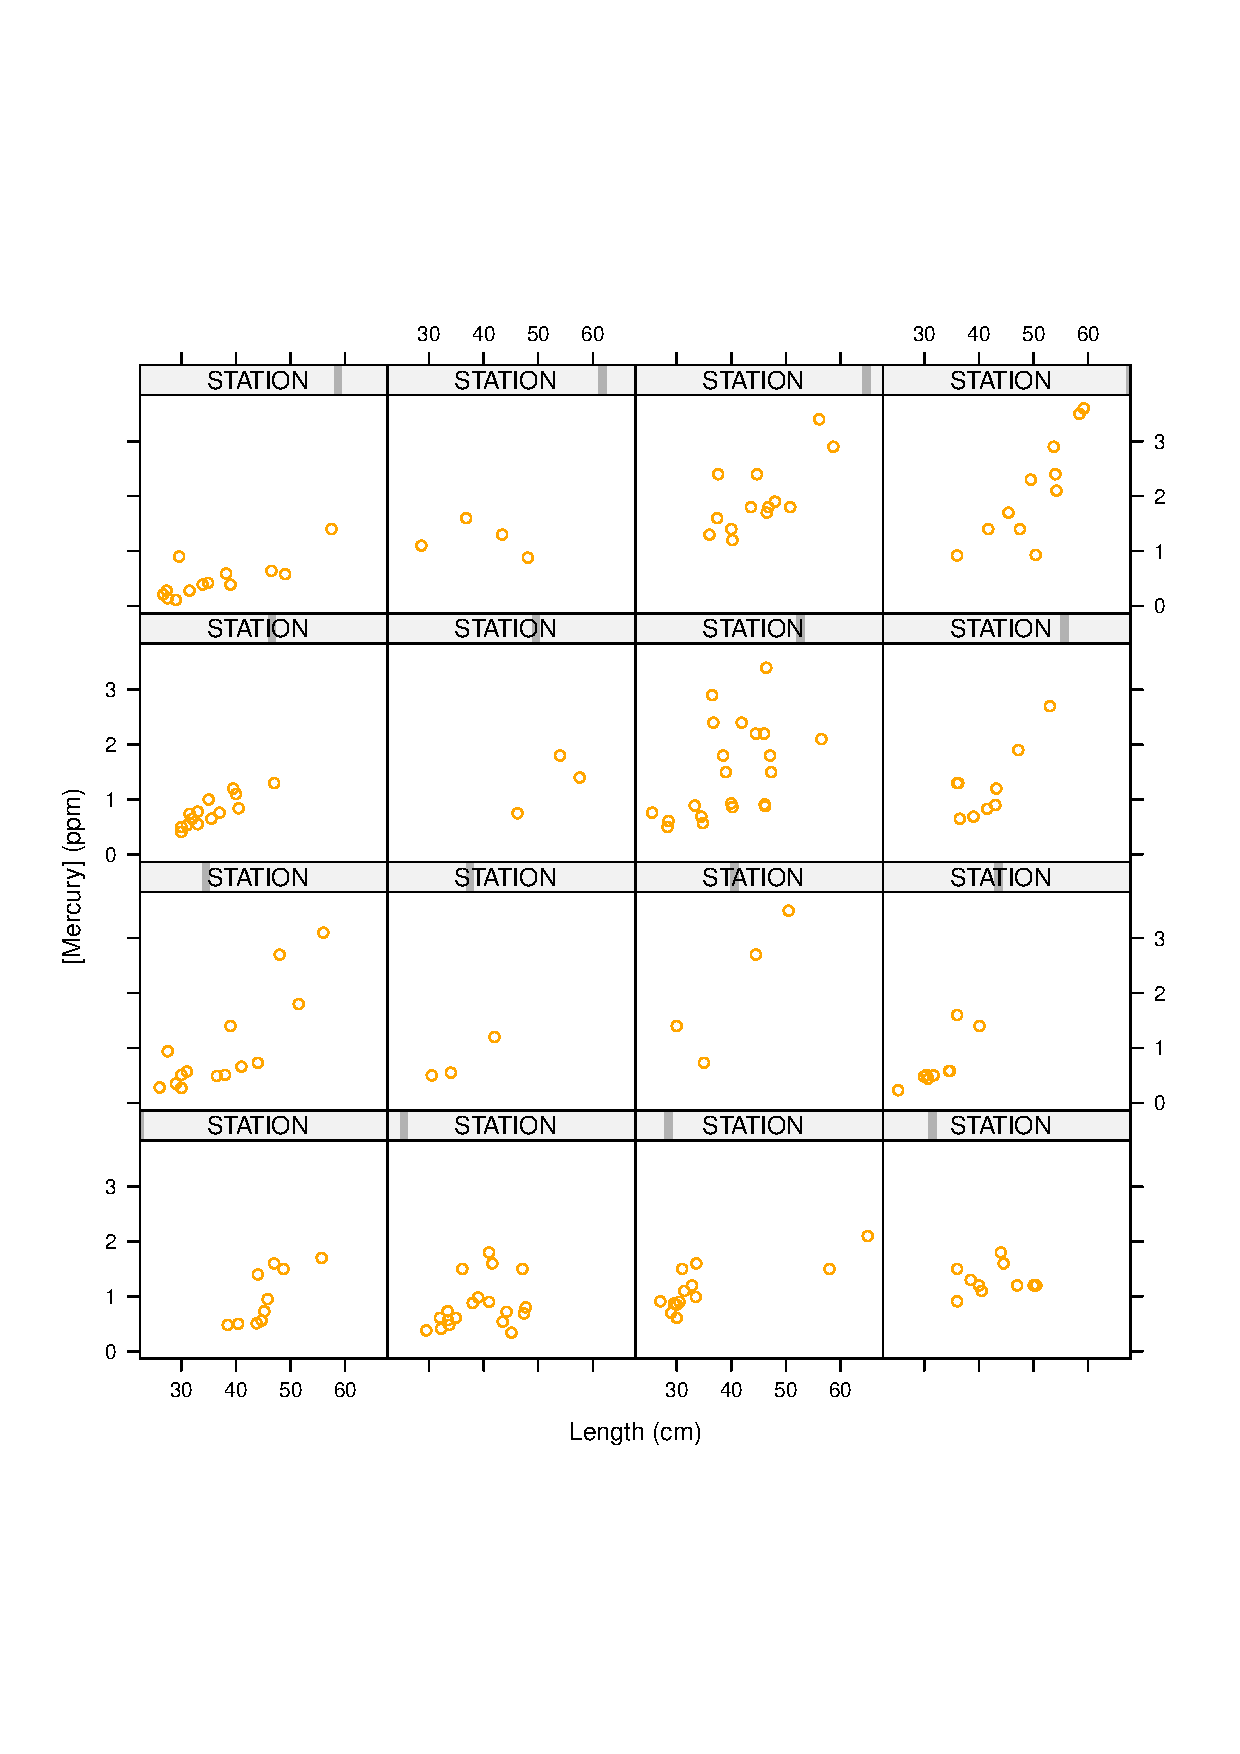
\includegraphics[height=3.5in]{fish-xy-smooth-lattice}
\end{frame}


\begin{frame}{Models}
Consider the following models for $\log{\M}$ as a function of
$\log{\L}$: \pause
\begin{enumerate}
\item  $\log{\M_{ij} = \beta_{0} + \beta_{1}\log \L_{ij}}$  (common
  line for all stations)  \pause
\item $\log{\M_{ij} = \beta_{0j} + \beta_{1}\log \L_{ij}}$  (parallel
  regression lines)  \pause

\item $\log{\M_{ij} = \beta_{0j} + \beta_{1j}\log \L_{ij}}$ (separate
  lines for each station)  \pause
\end{enumerate}
\vspace{.2in}
Use ANOVA to compare the 3 models
\end{frame}

\begin{frame}[fragile]
\frametitle{Fitting Models with Categorical Predictors in R}

\begin{verbatim}
fish$S = factor(fish$STATION) # convert to categorical
fish.com = lm(log(MERCURY) ~ 1 + log(LENGTH), data=fish)
fish.par = lm(log(MERCURY) ~ S + log(LENGTH), data=fish)
fish.dif = lm(log(MERCURY) ~ S*log(LENGTH), data=fish)
 
anova(fish.com, fish.par, fish.dif)
Analysis of Variance Table

Model 1: log(MERCURY) ~ 1 + log(LENGTH)
Model 2: log(MERCURY) ~ S + log(LENGTH)
Model 3: log(MERCURY) ~ S * log(LENGTH)
  Res.Df    RSS  Df Sum of Sq      F    Pr(>F)    
1    169 41.621                                   
2    154 23.974  15    17.648 8.1515 5.051e-13 ***
3    139 20.062  15     3.912 1.8070   0.03918 *  
---
Signif. codes:  0 '***' 0.001 '**' 0.01 '*' 0.05 '.' 0.1 ' ' 1 
\end{verbatim}
\end{frame}


\begin{frame}{Model Comparison: ANOVA Extra Sum-of-Squares F test}
    
Under all models the MSE = RSS/df under model (3) is an estimate of $\sigma^2$.
If one of the simpler models is true (say model (2)), then we expect that
the difference in RSS between model (2) and (3) will be small relative
to the extra degrees of freedom.
 \pause
Distribution of 
$$F_{obs} = \frac{\frac{RSS_{H_2} - RSS_{H_3}}{df_{H_2} -
    df_{H_3}}}{\hat{\sigma}^2_{H_3}} = \frac{\frac{ \Delta RSS}{\Delta
    df}}{\hat{\sigma}^2}$$
is an $F(df_{H_2} -   df_{H_3}, df_{H_3})$; compare the p-value = 
$P(F > F_{obs})$
 \pause
\vspace{.2in}
The ANOVA output suggests that we would 
\begin{itemize}
\item  reject model  (2) in favor of
(3) at the $\alpha = 0.05$ level, but not at the $0.01$ level  \pause
\item reject model (1) at any $\alpha > 5.05 \times 10^{-13}$
\end{itemize}
\end{frame}


\begin{frame}{Goals of Model}
  

  \begin{itemize}
  \item Model (3)  leads to a separate line for each of the 16
  stations 
 \pause
  \item Model (2) leads to a separate intercept for each of the 16 stations
  \end{itemize}
 \pause

How can we use these models to  predict $\M$ levels for other locations?
 \pause
\vspace{.2in}
View $\S$ as a random sample of locations and build a hierarchical
model \end{frame}

\begin{frame}[fragile]
\frametitle{JAGS/BUGS Model - Non-Centered}
\begin{verbatim}
for (n in 1:N){
 muj[n] <- alpha[station[n]]+beta[station[n]]*X[n]
 Y[n] ~ dnorm(muj[n], phi)
}

for (j in 1:J) {
  alpha[j] ~ dnorm(alpha.mu, alpha.phi)
  beta[j] ~ dnorm(beta.mu,  beta.phi)
}
phi ~ dgamma(.001, .001)
alpha.mu ~ dnorm(0.0, 1.0E-6)
alpha.sigma ~ dunif(0, 100)
alpha.phi <-1/(alpha.sigma*alpha.sigma)
beta.mu ~ dnorm(0.0, 1.0E-6)
beta.phi <- pow(beta.sigma, -2)
beta.sigma ~ dunif(0, 100)
\end{verbatim}
\end{frame}

\begin{frame}[fragile]
\frametitle{JAGS/BUGS Model - Centered}
\begin{verbatim}
for (n in 1:N){
 muj[n] <- alpha[station[n]]+beta[station[n]]*(X[n]-xbar)
 Y[n] ~ dnorm(muj[n], phi)
}

for (j in 1:J) {
  alpha[j] ~ dnorm(alpha.mu, alpha.phi)
  beta[j] ~ dnorm(beta.mu,  beta.phi)
}
phi ~ dgamma(.001, .001)
alpha.mu ~ dnorm(0.0, 1.0E-6)
alpha.sigma ~ dunif(0, 100)
alpha.phi <-1/(alpha.sigma*alpha.sigma)
beta.mu ~ dnorm(0.0, 1.0E-6)
beta.phi <- pow(beta.sigma, -2)
beta.sigma ~ dunif(0, 100)
\end{verbatim}
\end{frame}

\begin{frame}{Shrinkage}
       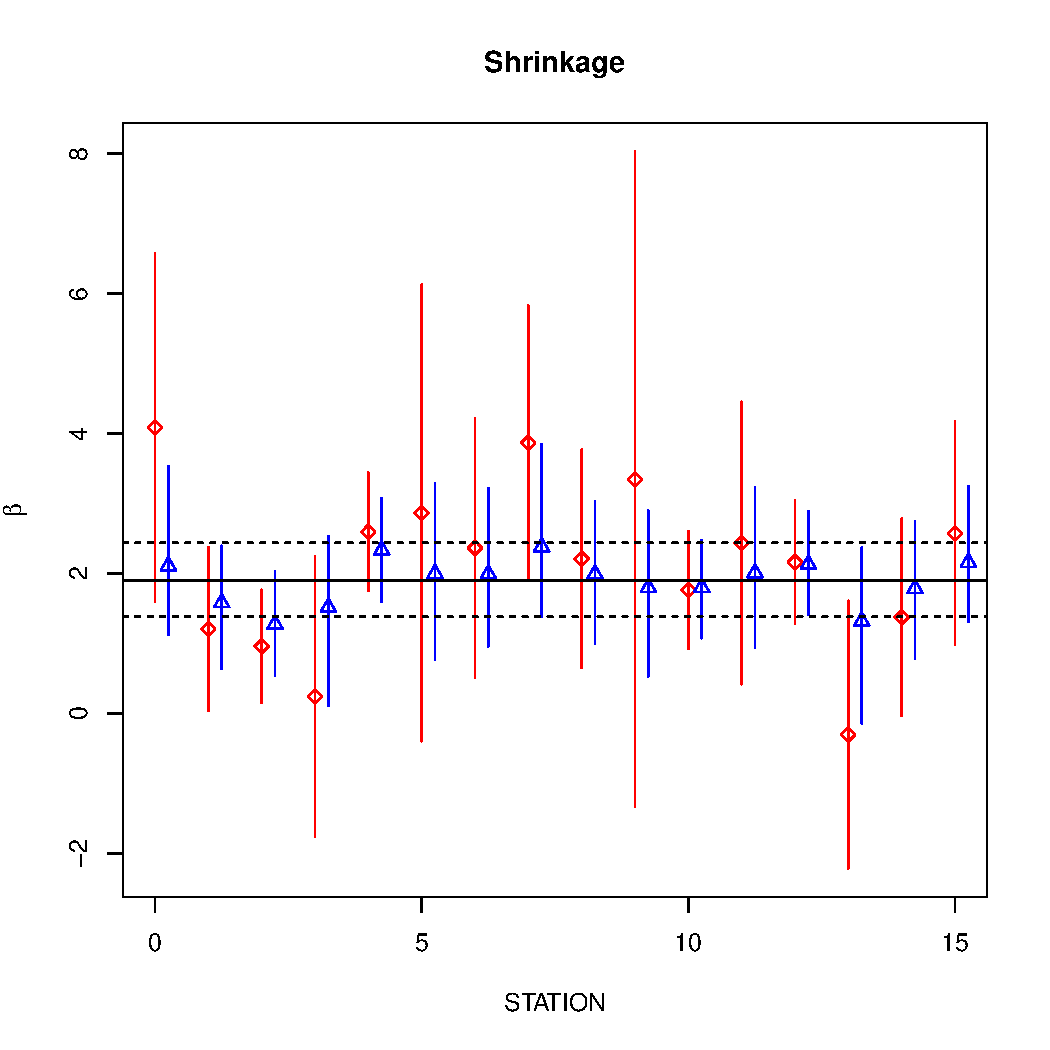
\includegraphics[height=3.5in]{shrinkage}
\end{frame}

\begin{frame}{Variance Components}
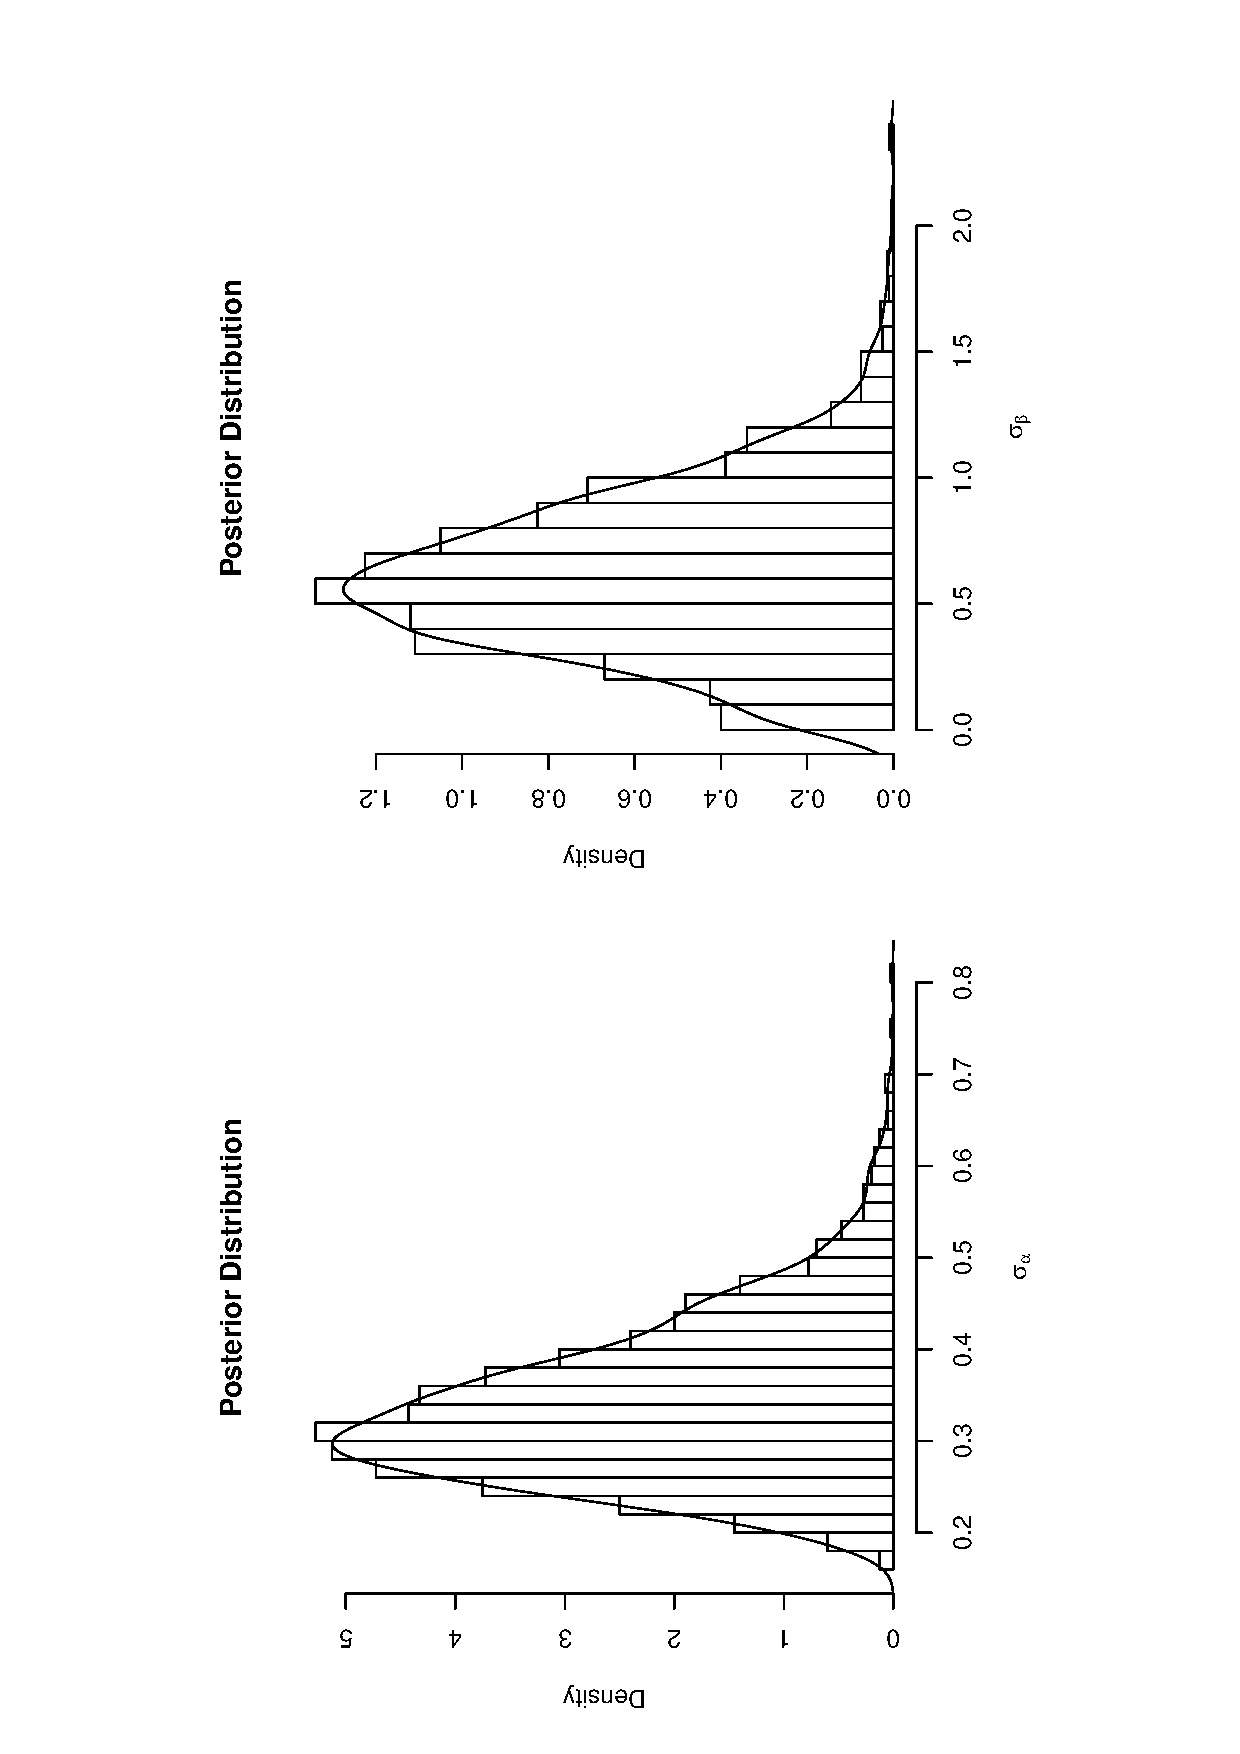
\includegraphics[height=2.5in]{varcomp}
\end{frame}

\begin{frame}{Interpretation of Coefficients}

\end{frame}
\begin{frame}{Percent Increase}
     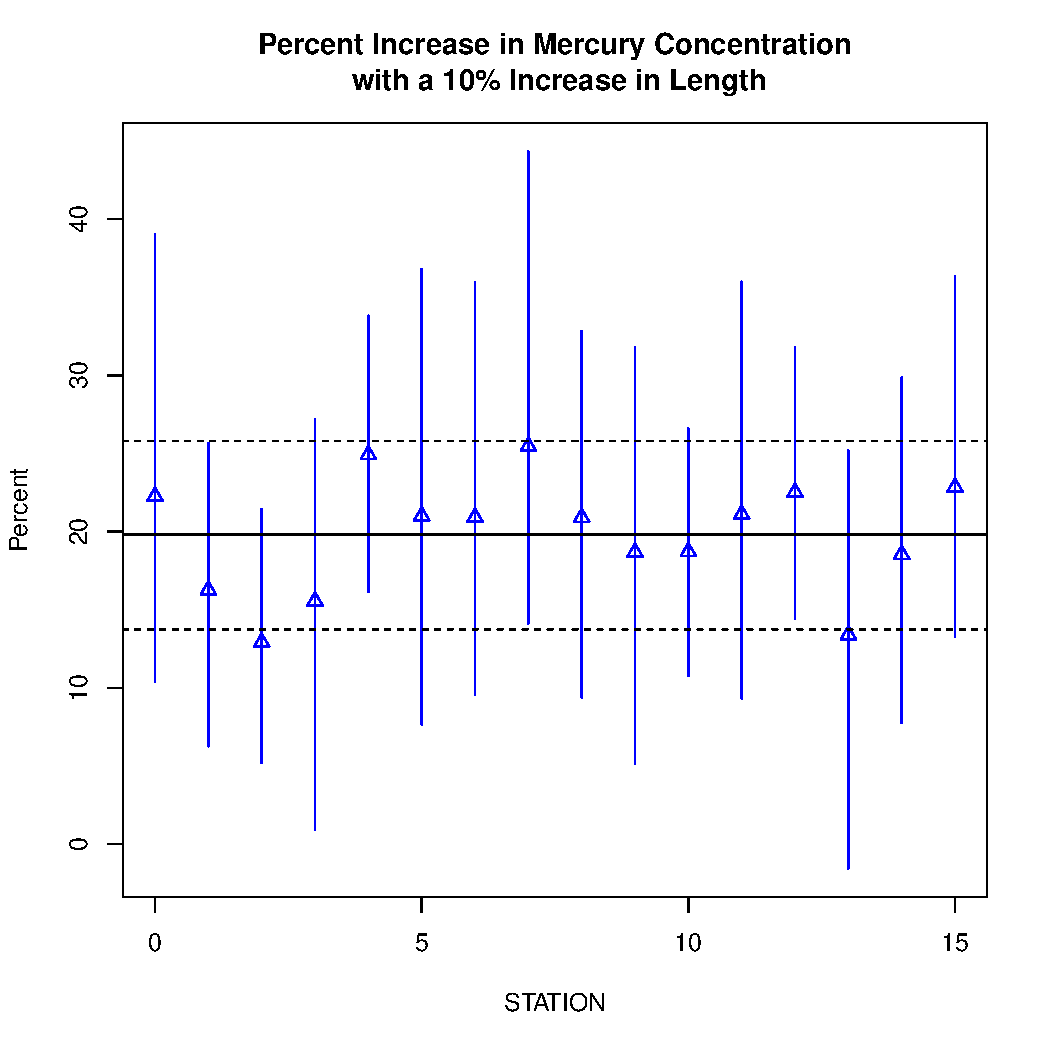
\includegraphics[height=3.5in]{increase}
\end{frame}
\begin{frame}{Predicting at a New Location}
\end{frame}

\begin{frame}{Predictions for a Random Location}
    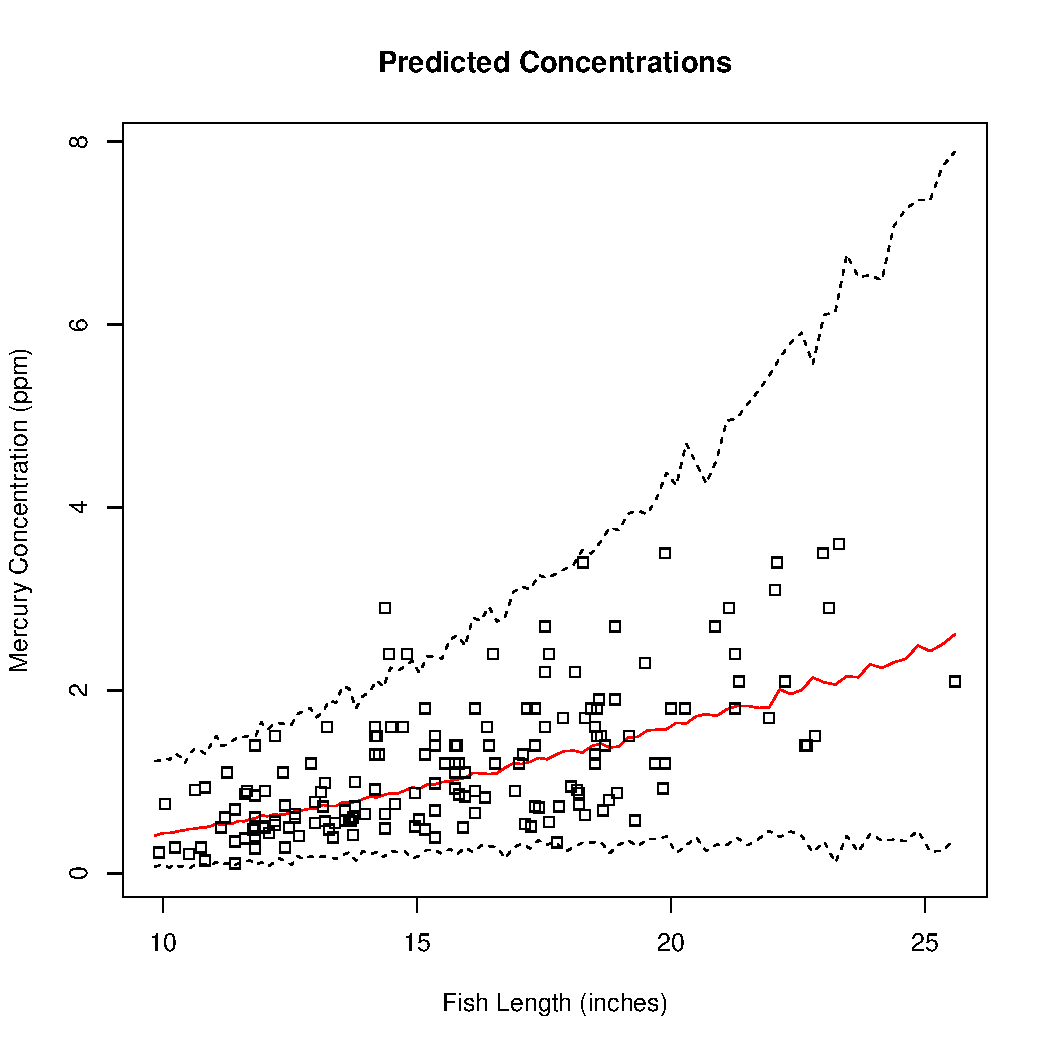
\includegraphics[height=3.5in]{pred}
\end{frame}

\begin{frame}{Probability Concentration Does not Exceed 1ppm}
  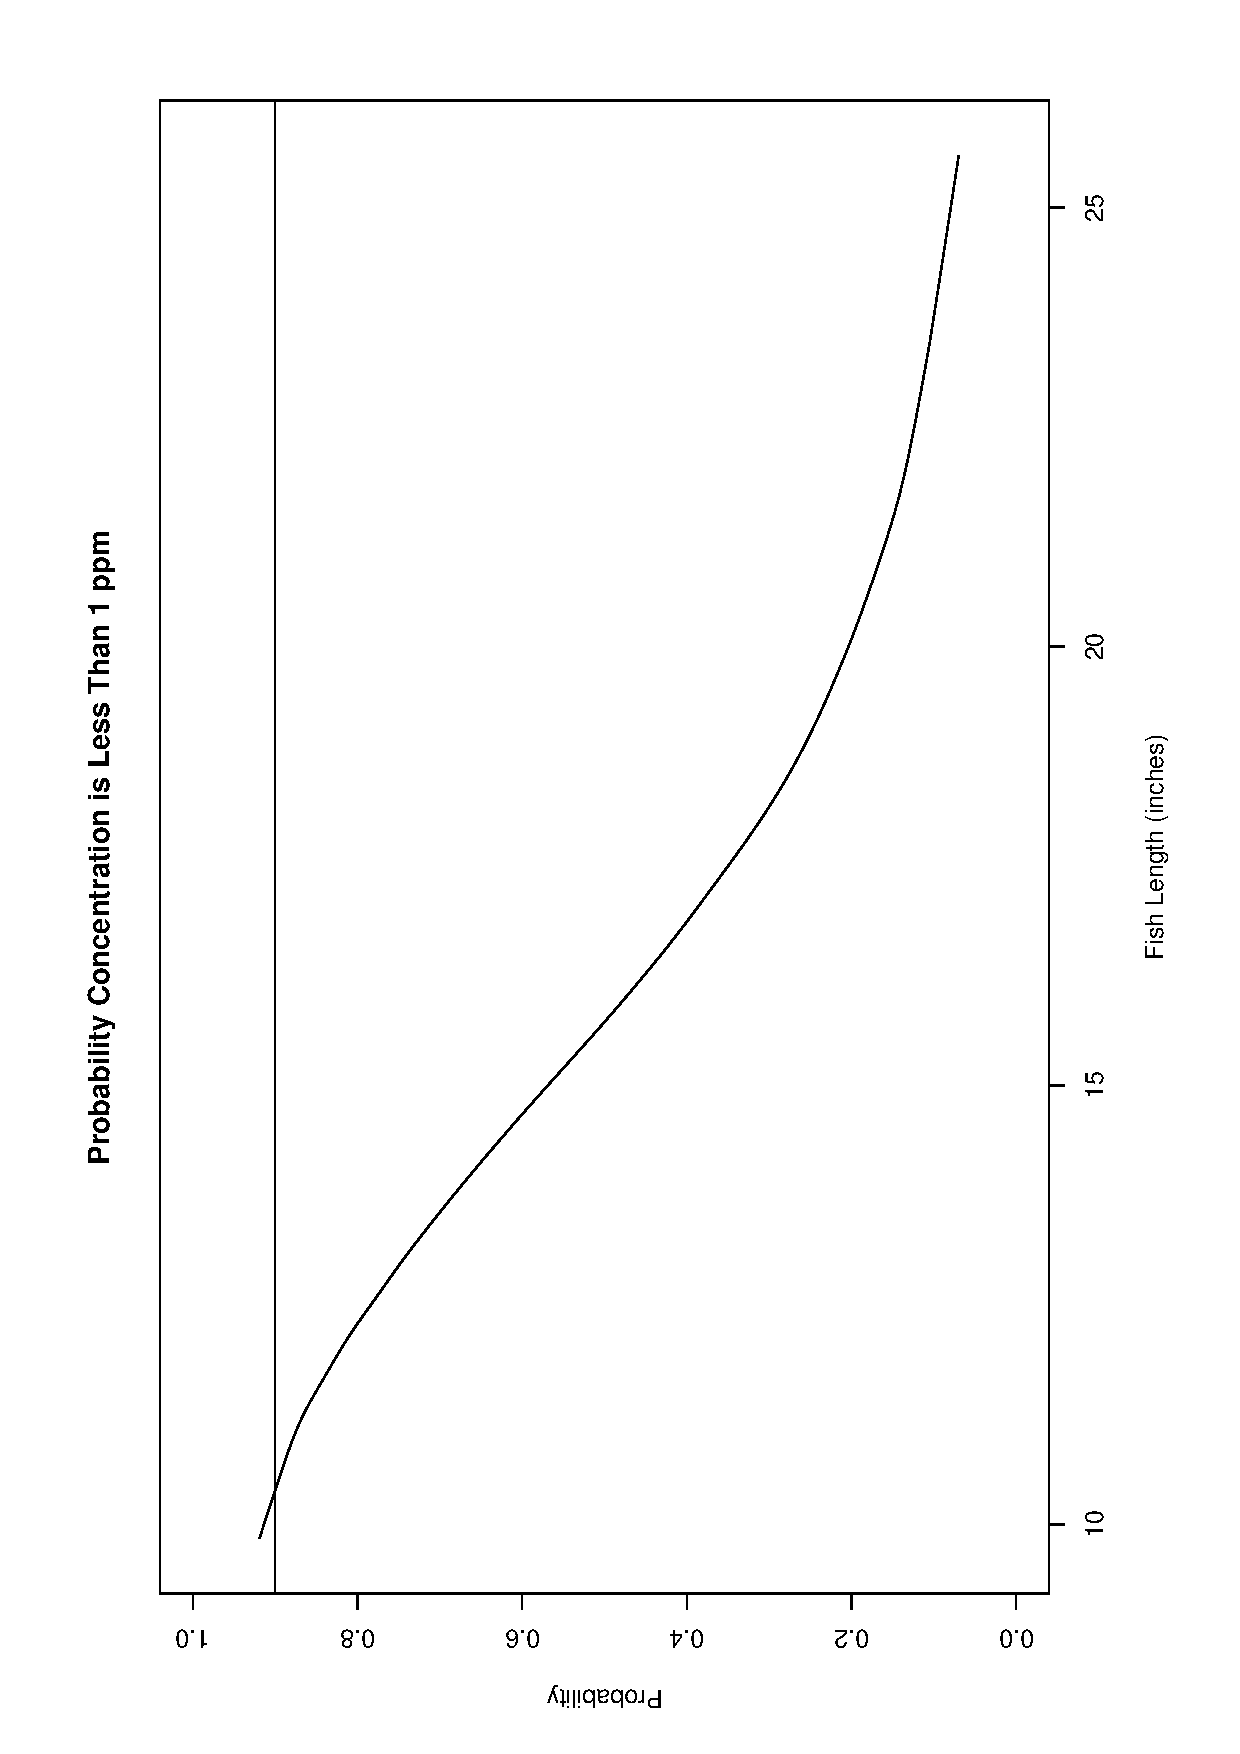
\includegraphics[height=3.5in]{prob}
\end{frame}


\begin{frame}{Model Extensions}
  \begin{itemize}
  \item Should intercepts or slopes depend on River?  Add another
  level to the hierarchy.  \pause
  \item Sensitivity of results to prior on variance components?  \pause
  Alternative prior distribution for standard deviation is a
  half-Cauchy.  (a Cauchy distribution restricted to $(0, \infty)$.
  \pause
\item Scaled Beta2 prior?  
  \item Inclusion of weight?  Measurement error model
  for weight as a function of length?   \pause
  \end{itemize}
  
\end{frame}
\end{document}

attach